\chapter{Modulares Eingabesystem}
\section{Schaltung}

Zur Umsetzung des Datenbusses wird für jedes Modul ein Mikrocontroller zur Kommunikation benötigt. 
Über die Mikrocontroller werden die zu verarbeitenden Eingangssignale vom jeweiligen Modul über den Bus an das Controller Modul übetragen. Für die 
unterschiedlichen Funktionen der Module, müssen jeweils andere Plantinen entwickelt werden. 

Für den ersten Prototypen werden ein Controller Modul unf ein Tastatur Modul entwickelt.


Da sich für das Busprotokoll an USB orientiert und um möglichst flexible und benutzerfreundliche Bedienung zu ermöglichen werden die Daten differentiell 
übertragen. So werden die Module sowohl modular über Federstecker und Magneten einfach aneinander anzuschließen sein, aber auch über eine Leitung, um die Benutzung flexibel zu machen.


\subsection{Controller Modul}
Der verwendete ESP ost wie in Abb. \ref{ESP} verschaltet.

\begin{figure}[H]
    \centering    
    \fbox{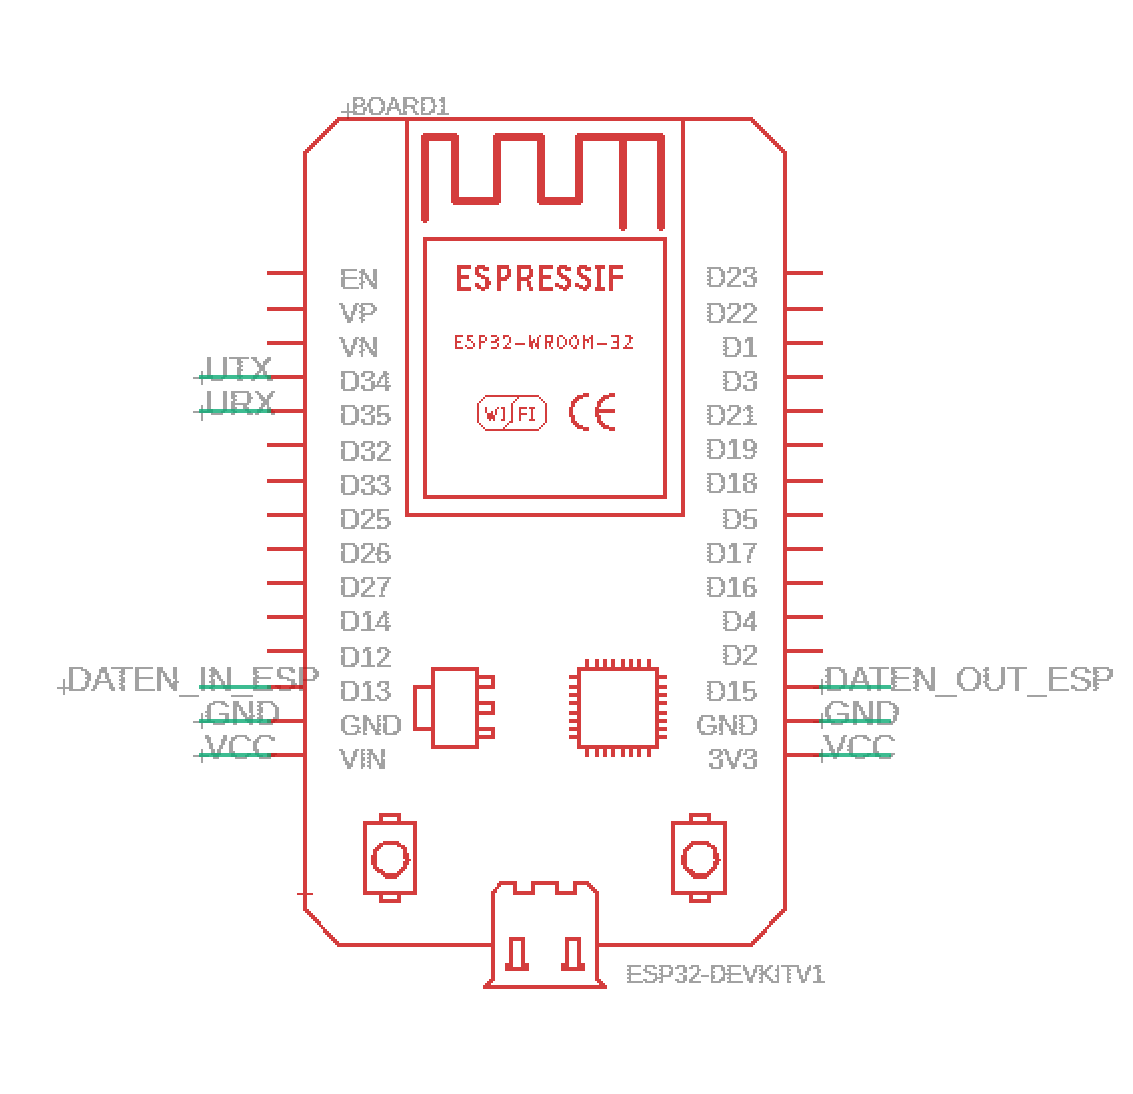
\includegraphics[width=.75\textwidth]{Bilder/BU_ESP.PNG}}
    \caption{ESP 32 Verschaltung}
    \label{ESP}
\end{figure}

Für die Kommunikation mit einem PC, werden die Daten über einen UART-to-USB Baustein gegeben, bevor sie an die USB Schnittstelle übertragen werden.


\begin{figure}[H]
    \centering    
    \fbox{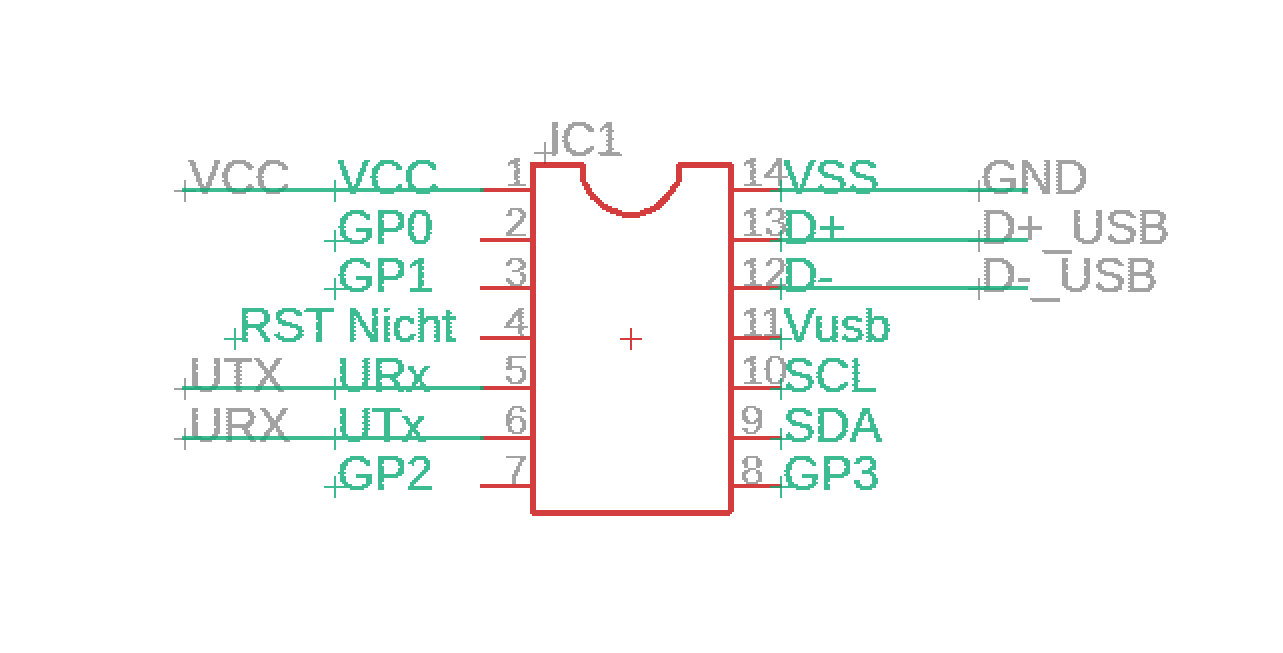
\includegraphics[width=.75\textwidth]{Bilder/BU_USB.PNG}}
    \caption{USB-to-UART}
    \label{USB}
\end{figure}

Zur Kommunikation mit den angeschlossenen Modulen, werden die Daten differnziell übertragen. Was, wie in Abb. \ref{T_R_Bausteine} dargestellt, 
über Transmit/receive Bausteine erfolgt.

\begin{figure}[H]
    \centering    
    \fbox{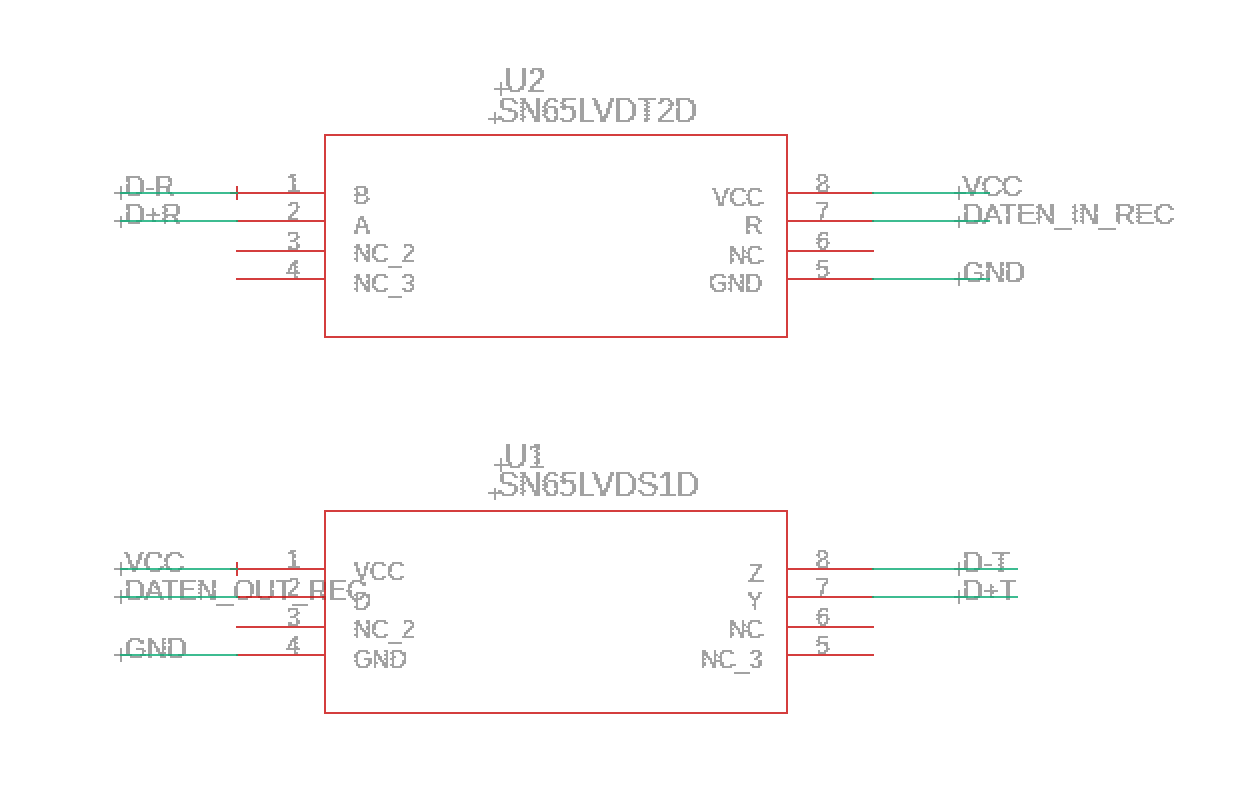
\includegraphics[width=.75\textwidth]{Bilder/BU_T_R_Bausteine.PNG}}
    \caption{Transmit- und Receive Bausteine}
    \label{T_R_Bausteine}
\end{figure}

\subsection{Tastatur Modul}
Das Tastatur Modul besteht aus 4x4 Tasten, die wie in \ref{Tastatur} zu sehen, verschaltet sind. Über vier Ausgänge des verwendeten AtMegas werden nacheinader 
Ausgangssignale gegeben, während über vier  Eingänge die Spalten abgefragt werden. Die Verschaltung des AtMegas ist in Abb. \ref{AtMega} zu sehen. Um das korrekte Auslesen zu gewährleisten, werden in jedem 
Ausgangspfad Schaltdioden eingesetzt. 
Der Mikrokontroller soll die Signale einlesen und sie über den Bus differenziell an das Controller Modul übertragen.


\begin{figure}[H]
    \centering    
    \fbox{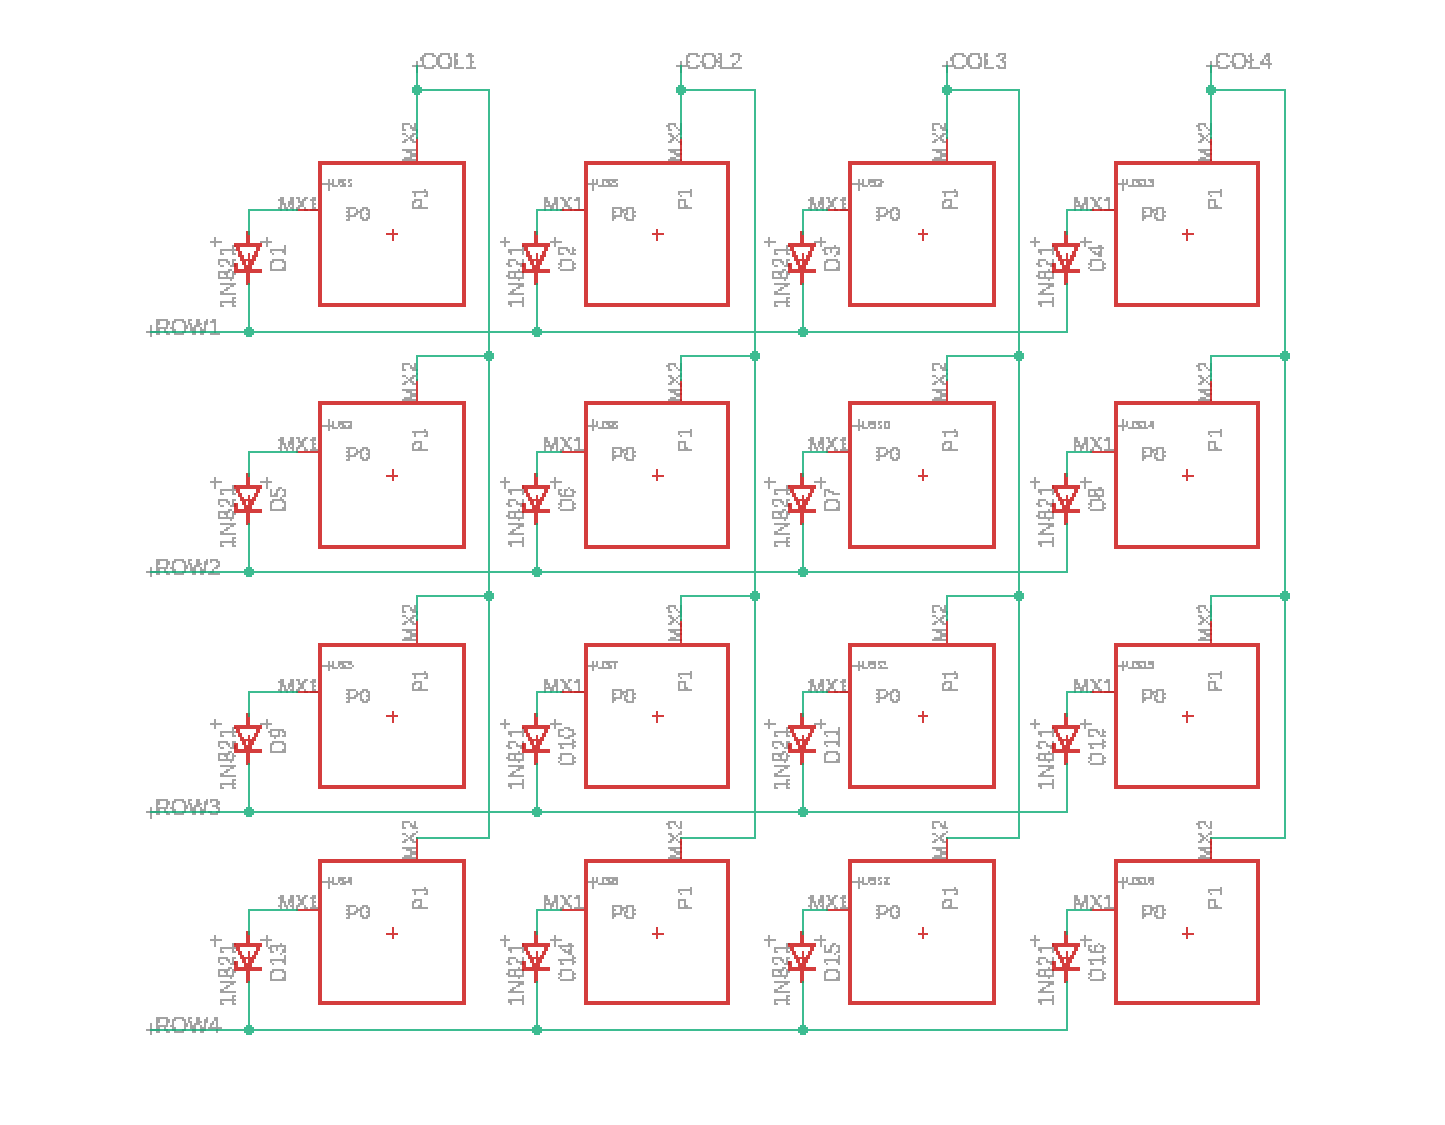
\includegraphics[width=.75\textwidth]{Bilder/BU_Tastatur.PNG}}
    \caption{Tastatur Schaltung}
    \label{Tastatur}
\end{figure}


\begin{figure}[H]
    \centering    
    \fbox{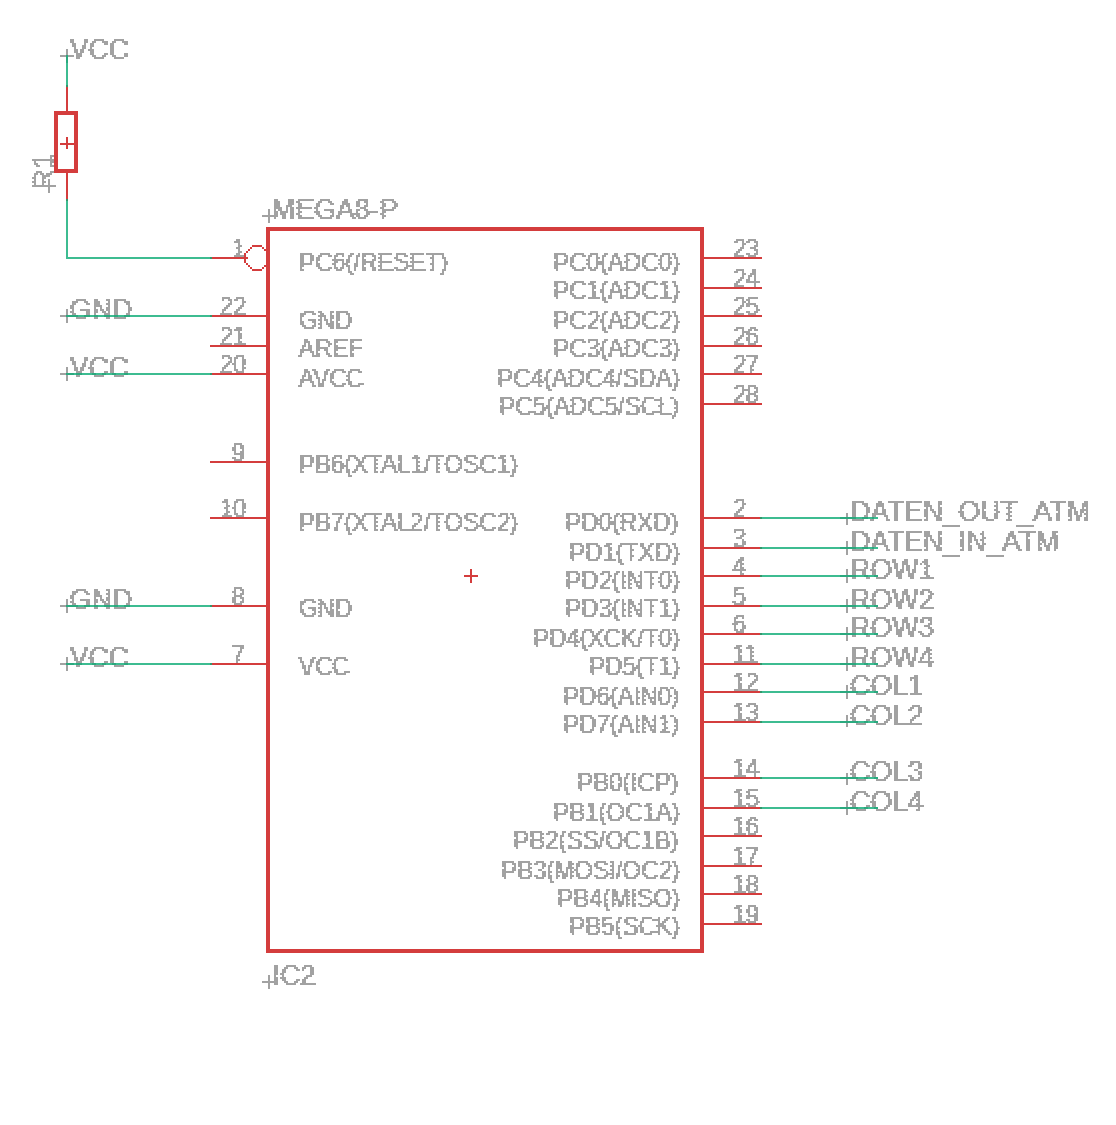
\includegraphics[width=.75\textwidth]{Bilder/BU_AtMega.PNG}}
    \caption{AtMega Verschaltung}
    \label{AtMega}
\end{figure}


\subsection{Testaufbau}


Da keine rechtzeitig lieferbaren Transmit-/ Receive ICs verfügbar waren, wurde der Testaufbau mit diskret aufgebauten Invertierern und Optokopplern gemacht.
Bei der Umsetzung kam es zu einigen zeitintensiven Schwierigkeiten. Da unwissentlich ein defekter Optokoppler verwendet wurde, war die Datenübertragung sowohl 
um den Faktor 1000 langsamer als im Datenblatt angegeben, als auch die Signalqualität war nicht geeignet. 
Nach einigem Suchen und testen von Alternativen, konnte eine funktionierende differenzielle Übertragung, wie in Abb. \ref{Optokoppler} 
aufgebaut werden. 
Aufgrund der Probleme bei der Realisierung wurde sich dazu entschieden auf dem Prototypen mehrere Möglichkeiten zur differenziellen Übertragung vorzusehen 
und über Jumper schalten zu können. 
Es wird die folgenden Möglichkeiten geben:

\begin{itemize}
\item nur die Transmit/Receive ICs zu verwenden,
\item die Transmit/Receive ICs mit zusätzlichen Optokopplern zu verwenden,
\item die Optokoppler mit diskret aufgebautem Invertierern und
\item das Umschalten auf eine Lochraster Platine für eventuelle Änderungen zu ermöglichen
\end{itemize}



\begin{figure}[H]
    \centering    
    \fbox{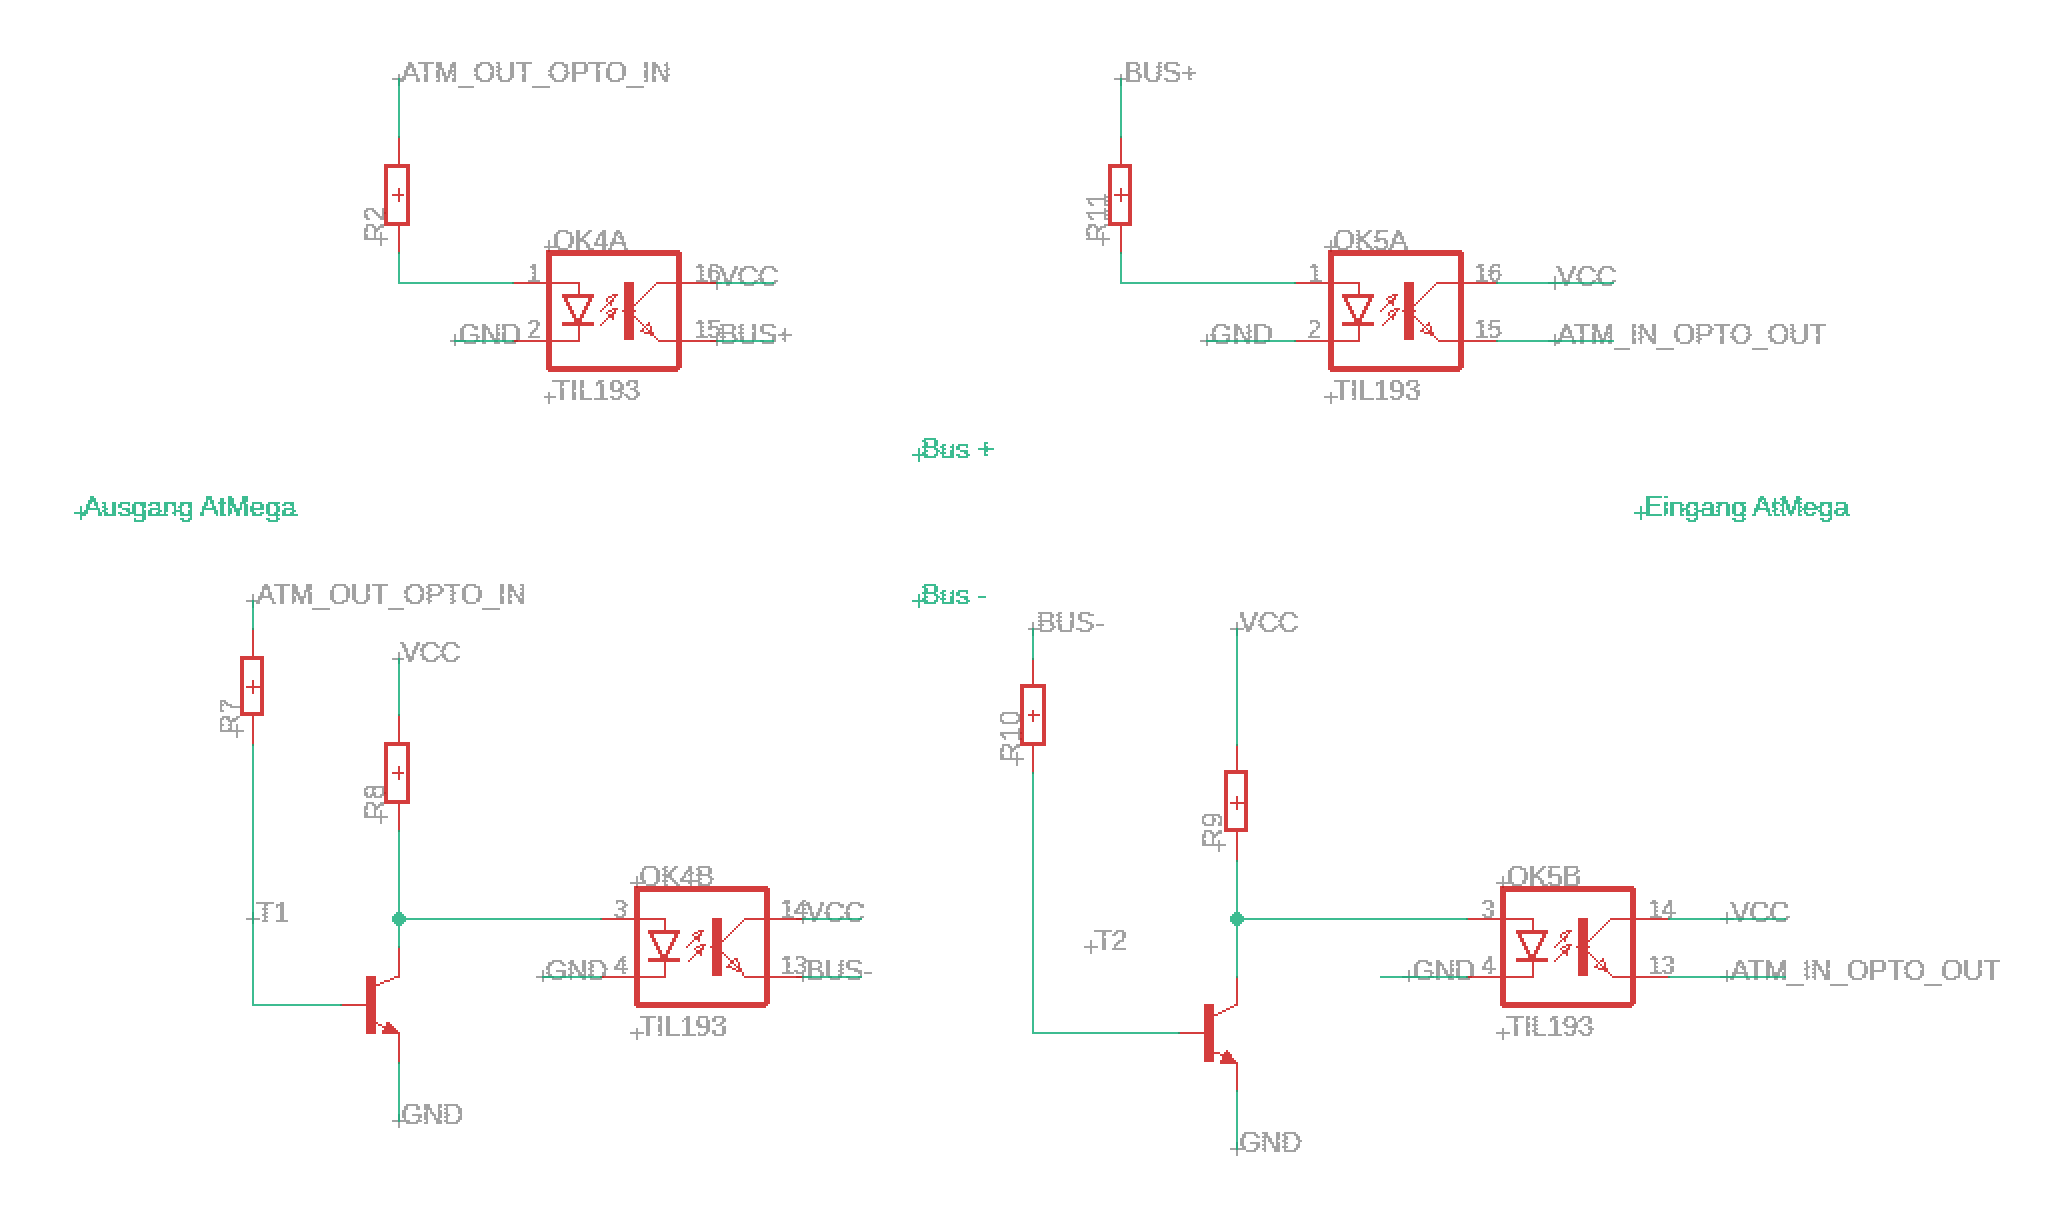
\includegraphics[width=.75\textwidth]{Bilder/BU_Optokoppler.PNG}}
    \caption{Optokoppler Schaltung}
    \label{Optokoppler}
\end{figure}




\section{Layout}







